\section{Motivation}

Modern hardware design is an immensely complex matter. Designs are getting
increasingly complex and there are a growing number of considerations to take.
To support further growth in performance, we need tools and methods that
facilitate a good design process where novel techniques can be prototyped
quickly.

\subsection{Historical Perspective}

Ever since the birth of computers, the world has seen an ever-increasing demand
for computing power. Computers have revolutionized our lives and become
fundamental for our society \cite{tanenbaum1984structured}. They have made it possible for
researchers to do simulations in great detail, helped the government to
streamline operations in healthcare and economics and made banking systems more
flexible. The Internet, made possible by computers, has had a massive impact on
how we live our lives; anyone with an Internet connection can exchange
information and communicate across land borders. Today, personal computers have
become ubiquitous and found uses ranging from home entertainment systems to
portable tablet computers. As applications in all these segments becomes richer,
the market demand for greater performance. Home users require higher frame
rates on their multimedia applications, researchers want more accurate
simulations for their experiments and the government will put better use to its
resources by processing more data.

Throughout the 80's and 90's, the increasing demand for performance was met by
increasing the clock frequency. Shortening the critical path and exploiting
instruction level parallelism allowed the CPU to run at higher clock speeds to
improve performance. Consequently, processor manufacturers were able to double
single-threaded performance approximately every 18th month
\cite{moore1965cramming}. The tradeoff, however, was an increased amount of
complex logic added complexity to the processor core. Greater complexity
required a greater amount of transistors which must fit on the same die, made
possible by the reduction of transistor size. For a long time, new process
technologies allowed for smaller and less energy consuming transistors, but as
we approached the end of Dennard scaling
\cite{dennard1974design,esmaeilzadeh2011dark}, the amount of logic required to
accomodate speedups could not fit on the die due to thermal constraints. Heat
generation on-chip became overwhelming and one could not simply increase the
frequency or add extra logic to gain additional performance.

\begin{figure}
    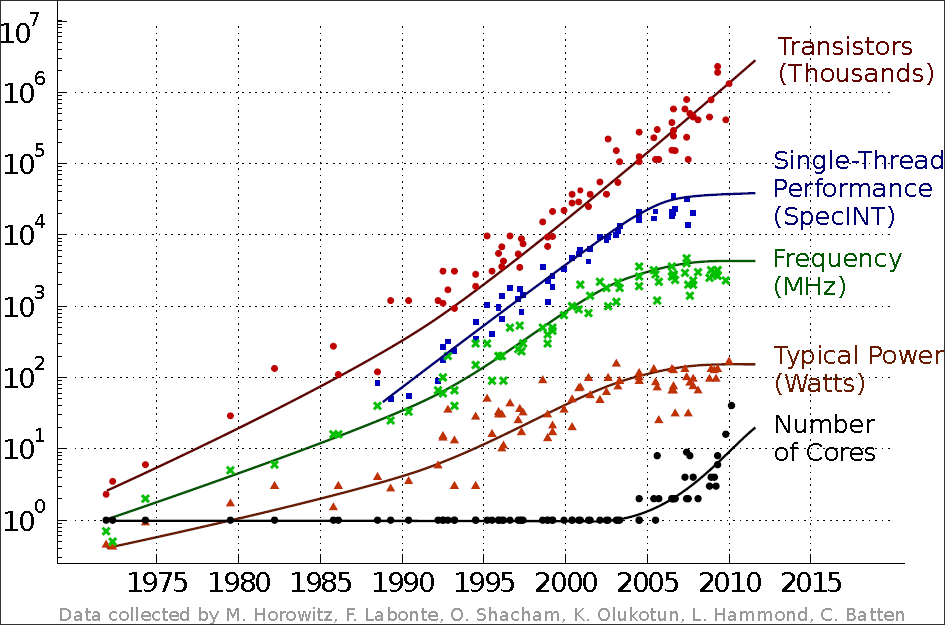
\includegraphics[width=\textwidth]{figs/cpu-performance.png}
    \caption{Historical trends in CPU performance, from \cite{salishan2011}.}
    \label{fig:cpuperformance}
\end{figure}

The tremendous growth in performance is depicted in
\autoref{fig:cpuperformance}. We note that although the transistor count is
steadily increasing, single-threaded performance has only seen a minor increase
the last few years.


\subsection{Problems of the New World}

Today's hardware designers are facing really hard problems. They must continue
to meet the market demand with respect to performance, while keeping the energy
consumption down. Energy consumption directly translates into heat generated
on-chip and is currently the limiting factor of processor design
\cite{hennessy}. Dealing with this requires hardware designers to emphasize
energy efficiency over pure performance during the design phase; we are entering
an era where a processor's performance per Watt is more important than
performance itself.

Heat is not the only motivation factor to keep energy consumption down.
Processors targeting laptops, cellphones and other mobile devices has always
been energy-constrained due to their use of batteries. Lower energy consumption
would allow for longer battery life and/or heavier applications. Processors in
this segment trades off performance in return of increased energy efficiency.
More recently, however, mobile processors has become increasingly popular in
alternative domains too, such as supercomputing. Their low cost and good
performance per Watt ratio makes them attractive for massively parallel
problems, which is currently done on large and expensive supercomputers. These
machines have huge energy budgets and are taken out of service after
just a couple of years, being replaced by new machines that offer better
performance for less power. For this reason, building datacenters from low-cost
embedded processors is believed to have a huge potential and change the
landscape of supercomputing the years to come.
%TODO: Add cite

Not only data centers benefit from the use of mobile processors. The SHMAC
research project at NTNU aims to build a single-ISA heterogeneous computing
platform with processing cores tailored to the application. Using the most
effective processor or hardware accelerator -- in terms of both energy
and performance -- is the key to success for such platforms.

There are great reasons to minimize a processor's energy consumption. Batteries
would last longer, applications become richer and it will enable processor
performance increase to continue. Thus, performance alone is no longer the most
important attribute of processors, energy efficiency is even more important.


\subsection{Better Tools for Optimizing Energy Efficiency}

Given the advanced tools used to support hardware design these days, it is more
easy than ever to model and simulate performance of an unimplemented
architecture. However, modeling power consumption is a much more elaborate
process: Current techniques works on a very low level and uses circuit-level
models to obtain energy metrics. This makes them accurate, but also heavy and
time consuming to simulate. Being able to rapidly prototype and visualize how
changes in the microarchitecture affects energy performance is a key to build
energy efficient hardware, and an important metric at the design stage. Some
solutions already exists, but most of them inspect energy consumption at very
fine granularity and requires ASIC synthesis of HDL code to work. During the
design process, there is a greater need for tools that help developers predict
the changes in power consumption when new features are implemented.

The immediate lack of a system that is easy to use and easy to set up motivates
the creation of a new high-level tool. We introduce PET; a tool that is able to
estimate power usage per time for a given workload on a given architecture. It
will use an energy metric profile estimated from similar processors together
with a simulator trace log to calculate energy usage. Using this approach, PET
will be able to detect if hardware modifications done to the simulation level
model will be beneficial in the realized hardware. PET will also tell if a
processor-implementation is more energy efficient than an other given a specific
workloads, thus it can help building workload optimized tiles for the SHMAC
project \cite{shmacwebpage}. Using the features of PET, one can also adjust the
energy metric profile and simulate power usage as if one component was cheaper
or more expensive to use (in terms of energy). This will enable hardware designers to
understand which optimizations are most beneficial and identify possible routes
of exploration in their journey of processor energy optimization.

% SHMAC, power profiles. Velg beste kjerne for gitt workload/application

% TODO: Introduce the notion of 'energy profiles', i.e. energy/time graphs

% motivation: early design stage, check architectural differences using same
% characteristics or set different weights to spesific events in the hunt for
% which components that needs optimization
